\subsection{Gram-Schmidt Orthogonalization Process}\label{subsec:Gram-Schmidt_Orthogonalization}
\begin{definition}[Span]\label{def:Span}
  The \emph{span} of a vector or set of vectors, is a linear combination of all possible vectors.
  For example, if $S = \lbrace u_{1}, u_{2} \rbrace$, then $\Span(S) = \lbrace c_{1}u_{1} + c_{2}u_{2} : c_{1}, c_{2} \in \RealNumbers \rbrace$.
\end{definition}

\begin{definition}[Projection]\label{def:Vector_Projection}
  The \emph{projection} of a vector onto another is the amount of one vector that is in the same direction as another.
  It is denoted $\Proj{u_{2}}{u_{1}}$, and is said ``the projection of $u_{2}$ on $u_{1}$''.
  It is defined as:
  \begin{equation}\label{eq:Vector_Projection}
    \Proj{u_{2}}{u_{1}} = \frac{u_{2} \cdot u_{1}}{u_{1} \cdot u_{1}} u_{1}
  \end{equation}
\end{definition}

\begin{definition}[Rejection]\label{def:Vector_Rejection}
  The \emph{rejection} of a vector from another vector is the amount that one vector is \textbf{not} in the same direction as another, in an orthogonal fashion.
  This can be seen graphically in \Cref{fig:Vector_Projection_Rejection}.
  It is denoted $\Rej{u_{2}}{u_{1}}$, and is said ``the rejection of $u_{2}$ from $u_{1}$''.
  If is defined as:
  \begin{equation}\label{eq:Vector_Rejection}
    \begin{aligned}
      \Rej{u_{2}}{u_{1}} &= u_{2} - \frac{u_{2} \cdot u_{1}}{u_{1} \cdot u_{1}} u_{1} \\
      \Rej{u_{2}}{u_{1}} &= u_{2} - \Proj{u_{2}}{u_{1}}
    \end{aligned}
  \end{equation}
\end{definition}

\begin{figure}[h!tbp]
  \centering
  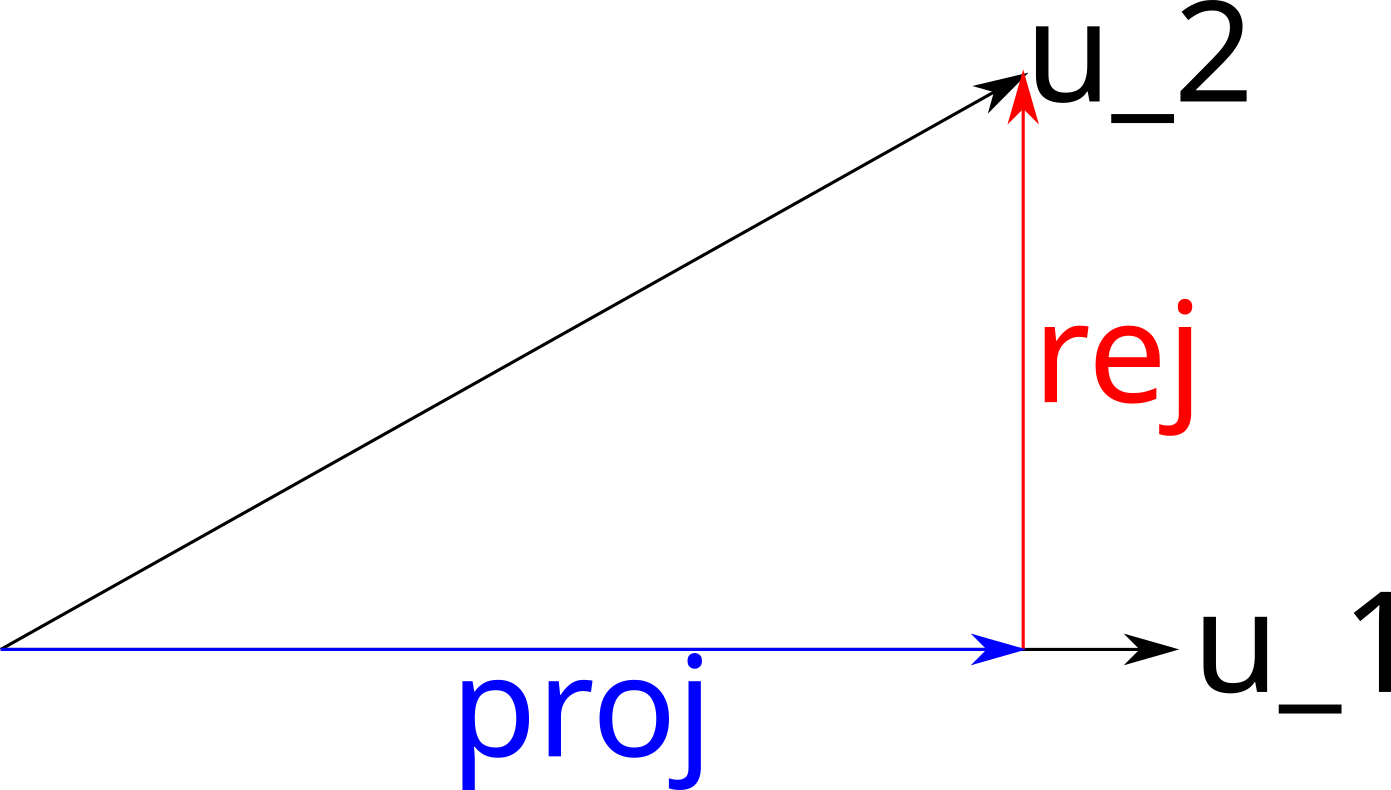
\includegraphics[scale=0.50]{./Vector_Projection_Rejection.png}
  \caption{Vector Projection and Rejection}
  \label{fig:Vector_Projection_Rejection}
\end{figure}


%%% Local Variables:
%%% mode: latex
%%% TeX-master: "../../Math_333-MatrixAlg_ComplexVars-Reference_Sheet"
%%% End:
